\documentclass{article}

\PassOptionsToPackage{numbers, compress}{natbib}
\usepackage[sglblindworkshop, final]{neurips_2026}
\workshoptitle{Predictive AI Evaluation Competition}

\usepackage[utf8]{inputenc}
\usepackage[T1]{fontenc}
\usepackage{hyperref}
\hypersetup{colorlinks=true, linkcolor=[rgb]{0.1,0.2,0.55}, citecolor=[rgb]{0.1,0.2,0.55}, urlcolor=[rgb]{0.1,0.2,0.55}}
\usepackage{url}
\usepackage{booktabs}
\usepackage{amsfonts}
\usepackage{amsmath}
\usepackage{nicefrac}
\usepackage{microtype}
\usepackage{xcolor}
\usepackage{graphicx}
\usepackage{enumitem}
\setlist{nosep, leftmargin=1.4em}

\newcommand{\ALC}{\mathrm{ALC}}

\title{Predicting AI-System Correctness on Unseen Benchmarks: Calibrated Hierarchical Adaptation and the Limits of Label-Only Prediction}

\author{%
  Satyajeeth Suresh Kannan\\
  Team BHopper\\
  Innovation Academy, Alpharetta, Georgia, USA\\
  \texttt{jeetusk08@gmail.com}
}

\begin{document}

\maketitle

\begin{abstract}
We predict whether an AI system answers an item of a never-seen benchmark correctly, before and after a few of its outcomes are
revealed. Our predictor is a hierarchical Bayesian logistic model with a benchmark level, a system effect, an item effect and
item-feature effects, fitted by MAP on every revealed label of the benchmark, with an item-text prior and a system prior from public
data. It needs only \texttt{numpy} and makes thousands of predictions in about a second. Three findings matter more than the model
class. First, our own formative feedback shows that the hidden benchmarks differ from the public ones: pair accuracies are spread
almost uniformly and benchmark levels vary far more than in the public data, which sets one prior width. Second, a faithful
re-implementation of the streaming evaluation and a simulator calibrated to the hidden pairs let us choose models without spending
leaderboard uploads. Third, we locate the limit of label-only prediction: for a system alone on its benchmark our predictor is within
0.0003~ALC of the Bayes-optimal level-only estimator, and the remaining 0.024~ALC gap to an oracle that knows each pair's accuracy
needs item-level knowledge that item text, sentence embeddings, small language-model states and perplexity did not supply across
benchmarks. We also show that practice-board differences largely track how many times a team uploaded, because each upload is
scored on 9 sampled pairs and the board keeps a team's best score.
\end{abstract}

\section{Introduction}

The competition~\cite{paiec} asks for a program that predicts $P(\text{correct})$ for an AI system $s$ on an item $i$ of a benchmark that was
not in the training pool, first with no outcomes of that system on that benchmark and then after 1, 3, 7, 15 and 31 of them have been
revealed. Predictions are scored by Brier score~\cite{brier1950} at each budget. The setting is close to item response
theory~\cite{rasch1960} and to efficient evaluation with few items~\cite{polo2024tiny}, with two differences that drive everything
below: the benchmark is new, so item parameters cannot be learned in advance, and the evaluation is streaming, so a method
has to adapt from very few labels.

Our contributions are:
\begin{itemize}
  \item A numpy-only hierarchical predictor (Section~\ref{sec:method}) that is calibrated for the hidden test's structure, which we
        infer from our own formative feedback without identifying any hidden benchmark (Section~\ref{sec:data}).
  \item Three model-selection tools that replace leaderboard probing (Section~\ref{sec:selection}), including a faithful
        re-implementation of the official streaming protocol.
  \item A measured limit: for a lone system the predictor is at the Bayes limit of label-only prediction, and the remaining gap needs
        item-level knowledge that did not transfer across public benchmarks in any form we tested (Sections~\ref{sec:results}
        and~\ref{sec:negative}).
  \item An analysis of what the practice board measures (Section~\ref{sec:board}).
\end{itemize}

\paragraph{Selected submission.} Version v6 (\texttt{paie\_v6.zip}, SHA-256
\texttt{45c6596a\ldots 7aea08}, full hash in Appendix~\ref{app:repro}), uploaded to Codabench on 28 September 2026 as submission \#949120. Version v7 (Section~\ref{sec:v7}) adds an acquisition rule with a consistent but
negligible gain; it is not selected because it has not been run on the platform, and a gain of at most 0.0005~ALC does not
justify that risk.

\section{Task, interface and metric}
\label{sec:task}

The program is called as \texttt{predict([subject, item], labeled)}. The \texttt{subject} has eight string fields
(\texttt{normalized\_name}, \texttt{provider}, \texttt{release\_date}, \texttt{access\_date}, \texttt{harness},
\texttt{harness\_version}, \texttt{reasoning\_effort}, \texttt{subject\_features\_extra}). The \texttt{item} has
\texttt{item\_content}, \texttt{item\_features}, \texttt{interactors} and an anonymous benchmark ID; there is no reference answer and no
benchmark name. \texttt{labeled} holds every outcome revealed so far, for all sampled subject--benchmark pairs.

Each pair with at least 80 items is split 50/50 into an acquisition pool and an evaluation pool, independently for each pair. An
optional acquisition function sees candidates in a fixed random order; without one, labels are drawn at random. Predictions on the
evaluation pool are scored by Brier score $B_k$ at budgets $k \in \{0,1,3,7,15,31\}$ and combined as
\begin{equation}
  \ALC = 0.1\,B_0 + 0.2\,(B_1 + B_3 + B_7 + B_{15}) + 0.1\,B_{31},
\end{equation}
averaged equally over pairs (lower is better). Evaluation workers are recreated at each budget, so no state survives between budgets;
this costs nothing because \texttt{labeled} is complete in every call. When two systems share a benchmark, one system's labels can
fall on the other's evaluation items. This is the only source of item-specific evidence inside the evaluation.

\section{Data, and what the hidden test looks like}
\label{sec:data}

\paragraph{Public training pool.} \texttt{measurement-db}~\cite{measurementdb} has 6 benchmarks and 227{,}995 system--item pairs
with up to 200 trials per pair: matharena (104 systems, 1{,}755 items), mmdocrag (68, 2{,}000), multi\_swebench (82, 2{,}078),
real\_webagents (33, 233), researchcodebench (31, 212) and swe\_rebench (1, 6{,}271).

\paragraph{Where the predictable variance is.} Table~\ref{tab:oracle} compares a constant equal to the benchmark mean with three
oracles: the true per-system accuracy, the true per-item accuracy, and an additive logistic (Rasch) fit. On five of six benchmarks,
knowing item difficulty removes more error than knowing system strength.

\begin{table}[h]
  \caption{Oracle Brier scores per public benchmark (trial-level, in-sample on the full data; Rasch: additive logistic fit, ridge
  0.01; lower is better).}
  \label{tab:oracle}
  \centering\small
  \begin{tabular}{lcccc}
    \toprule
    Benchmark & Benchmark mean & Subject oracle & Item oracle & Rasch oracle \\
    \midrule
    matharena          & 0.210 & 0.180 & 0.109 & 0.075 \\
    mmdocrag           & 0.173 & 0.132 & 0.148 & 0.101 \\
    multi\_swebench    & 0.128 & 0.106 & 0.068 & 0.057 \\
    real\_webagents    & 0.234 & 0.186 & 0.134 & 0.094 \\
    researchcodebench  & 0.228 & 0.205 & 0.130 & 0.090 \\
    swe\_rebench       & 0.249 & 0.249 & 0.045 & 0.046 \\
    \bottomrule
  \end{tabular}
\end{table}

\paragraph{The hidden test, inferred from our own formative feedback.} Every model predicts 0.5 at budget 0, so the one-bin budget-0
calibration error equals $|0.5 - \bar y|$, which gives each scored pair's accuracy up to reflection. Our three scored uploads cover
26 pairs on 7 hidden benchmarks. Each sample has 9 pairs: every benchmark appears once and two of them have a second system; no system
appears on two benchmarks within a sample. We find that (i) pair accuracies are spread like Uniform(0,1)
($\mathbb{E}[\bar y(1-\bar y)] = 0.162$, against 0.167 for a uniform distribution); (ii) hidden benchmarks differ from each other much
more than public ones (rms logit accuracy 1.70 vs.\ 1.08); and (iii) systems within a hidden benchmark are similar (sd 0.2--1.1 logit
including sampling noise, 0.2--0.7 on 6 of the 7 benchmarks). These numbers are used only to set one global prior width and to build
a synthetic validation set. No model uses a benchmark-specific value, and we made no attempt to identify the benchmarks behind the
anonymous IDs.

\section{Method (submission v6)}
\label{sec:method}

The model is
\begin{equation}
  \operatorname{logit} p(s,i) = \beta_b + \delta_s + \varepsilon_i + G_i^\top g,
\end{equation}
fitted per benchmark $b$ by three block-Newton MAP sweeps on all labels revealed for that benchmark. Every system that shares the
benchmark pools its labels, and items are matched by their full visible description. The priors are listed in
Table~\ref{tab:priors}.

\begin{table}[h]
  \caption{Priors of the v6 model.}
  \label{tab:priors}
  \centering\small
  \begin{tabular}{lll}
    \toprule
    Term & Prior & Detail \\
    \midrule
    Benchmark level $\beta_b$ & $\mathcal{N}(0, \tau_b^2)$, $\tau_b = 1.4$ & wide, because hidden benchmark levels are spread \\
    System effect $\delta_s$ & $\mathcal{N}(m_s, \tau_s^2)$, $\tau_s = 0.8$ & $m_s$: half the system's relative strength on public data$^{a}$ \\
    Item effect $\varepsilon_i$ & $\mathcal{N}(m_i, \tau_i^2)$, $\tau_i = 1.5$ & $m_i$: hashed word uni+bigram TF-IDF dual ridge$^{b}$ \\
    Item features $g$ & $\mathcal{N}(0, \tau_g^2)$, $\tau_g = 0.5$ & one-hot \texttt{item\_features} tokens, z-scored numerics$^{c}$ \\
    \bottomrule
  \end{tabular}\\[2pt]
  \raggedright\footnotesize
  $^{a}$ Logit accuracy minus the benchmark mean, matched by normalised model name; fallback: a ridge on metadata (release date,
  provider, size and variant tokens, reasoning effort). Name-matched systems recur across public benchmarks with strength
  correlations of $+0.23$ to $+0.90$.
  $^{b}$ Fitted to the labelled items' effects of the same benchmark and refitted three times.
  $^{c}$ Tokens shared by at least two labelled items, plus a slope per numeric key clipped to $\pm 3$.
\end{table}

At budget 0, or when the benchmark has no label, the prediction is 0.5 (Section~\ref{sec:negative} explains why nothing better
transferred). Soft labels are used as given; malformed input never raises, and the fallback is a smoothed pair mean, then 0.5. The
code uses \texttt{numpy} and the standard library only and is deterministic: 3{,}000 predictions with 1{,}860 labels on
$\sim$100\,KB items take 1.1\,s on a laptop CPU.

\section{Choosing models without the leaderboard}
\label{sec:selection}

\begin{enumerate}
  \item \textbf{Leave-one-benchmark-out harness} on the public data (fractional labels, 3 seeds), with four regimes: \emph{single}
        (each system alone), \emph{mix2}, \emph{mix8} and \emph{pooled} (all systems of the held-out benchmark).
  \item \textbf{Faithful streaming simulator.} It drives any submission through the official call shapes, reconstructed from the
        organisers' ingestion code: per-pair splits, the evaluator's own random acquisition rule, worker re-creation at each budget,
        binary labels, and a per-fold subject prior rebuilt without the held-out benchmark. Regimes: \emph{practice} (1--2 systems
        of the held-out benchmark plus one filler pair from every other benchmark) and \emph{kN} ($N$ systems of the held-out
        benchmark).
  \item \textbf{Hidden-calibrated simulator.} It rebuilds our three dev samples, or fresh samples with the same structure, from each
        pair's accuracy. Item effects follow a Rasch model ($\tau_{\text{true}}$ 1.0--2.0) shared by the systems of a benchmark. Item
        texts are random, so there is no text signal.
\end{enumerate}

\section{Results}
\label{sec:results}

\paragraph{Development history.} Table~\ref{tab:history} shows the leave-one-benchmark-out harness. The single regime is about
0.025~ALC harder, because item difficulty can only come from the system's own labels. (This harness omitted a $-\beta/\tau_b^2$ prior
term that the shipped v5 contains; re-measured as shipped, v5 scores 0.1874 single and 0.1627 pooled.)

\begin{table}[h]
  \caption{Leave-one-benchmark-out ALC on the public data (lower is better).}
  \label{tab:history}
  \centering\small
  \begin{tabular}{lcc}
    \toprule
    Model & Pooled & Single \\
    \midrule
    Organisers' empirical-mean baseline (replicated) & 0.216 & 0.216 \\
    Pooled hierarchical, flat prior (v1) & 0.169 & -- \\
    + item-text prior (v2) & 0.161 & 0.186 \\
    + name-matched system prior, MAP fit, $\tau = 1.0$ (v3) & 0.161 & 0.188 \\
    $\tau = 0.8$, system prior $\times 0.5$ (v5) & 0.162 & 0.186 \\
    \bottomrule
  \end{tabular}
\end{table}

\paragraph{From v5 to v6.} v6 raises $\tau_b$ from 0.8 to 1.4 (so a lone system's benchmark level adapts faster), adds the
item-feature group effects and hardens the code. Table~\ref{tab:v5v6} shows that it is clearly better for a lone system, which is the
practice-board case, and about equal when many systems pool their labels. Not every benchmark improves: researchcodebench is slightly
worse in every harness regime (single $+0.0016$), and in the pooled regime v6 improves only 2 of 6 benchmarks.

\begin{table}[h]
  \caption{v5 (previous submission, as shipped) vs.\ v6 in the three tools (ALC, lower is better).}
  \label{tab:v5v6}
  \centering\footnotesize
  \begin{tabular}{lcc}
    \toprule
    Tool and regime & v5 & v6 \\
    \midrule
    Harness: single (3 seeds) / mix2 & 0.1874 / 0.1841 & \textbf{0.1854} / \textbf{0.1828} \\
    Harness: mix8 / pooled & 0.1770 / 0.1627 & 0.1772 / 0.1634 \\
    Faithful simulator: practice (pair-weighted) & 0.2051 & \textbf{0.2024} \\
    Faithful simulator: k1 / k2 & 0.2128 / 0.2068 & \textbf{0.2111 / 0.2062} \\
    Faithful simulator: k4 / k8 & 0.1991 / 0.1916 & \textbf{0.1987 / 0.1915} \\
    Hidden-calibrated: practice samples ($\tau_{\text{true}}$ 1.5) & 0.1957 & \textbf{0.1918} \\
    Hidden-calibrated: 8 systems per benchmark (sd 0.4 / 0.8) & 0.1778 / 0.1782 & \textbf{0.1752 / 0.1765} \\
    \bottomrule
  \end{tabular}
\end{table}

\begin{figure}[t]
  \centering
  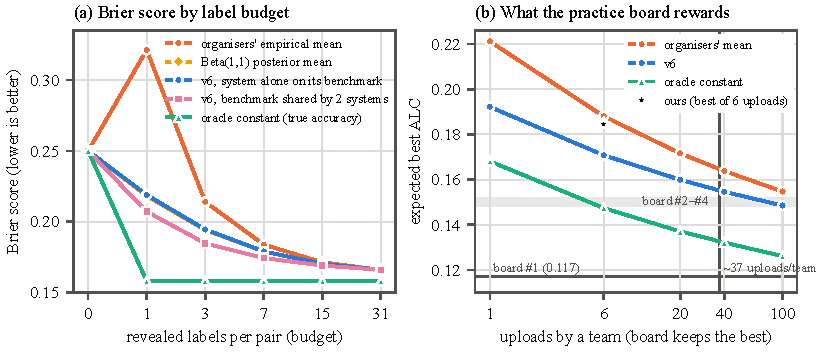
\includegraphics[width=\linewidth]{fig_curves.pdf}
  \caption{Hidden-calibrated simulator, 1{,}800 fresh 9-pair samples. (a) Brier score at each label budget; the Beta(1,1) curve lies
  under the v6 lone-system curve. The unsmoothed empirical mean loses most at $B_1$, where one label sets its prediction to 0 or 1.
  (b) Expected best practice-board score of a team that uploads $N$ times, with the board as read on 7 October 2026 (\#1, the band
  of \#2--\#4, our best of 6 uploads, and the mean number of uploads per team).}
  \label{fig:curves}
\end{figure}

\paragraph{For a lone system, v6 is at the Bayes limit of label-only prediction.} After $k$ labels, a lone system's labels say only
``$m$ of $k$ correct''. Without item-level knowledge every unlabelled item looks the same, so the Bayes-optimal prediction is the
posterior mean of the pair accuracy; with the near-uniform hidden accuracy distribution this is close to the Beta(1,1) posterior
mean $(m+1)/(k+2)$. Figure~\ref{fig:curves}a and Table~\ref{tab:bayes} show that v6 matches it on lone pairs (a more U-shaped
Beta(0.7,0.7) prior is not better), and that v6's whole gain over Beta(1,1) comes from pairs that share a benchmark, where the second
system's labels inform the level and, through shared item effects, the very items being predicted. Per sample, v6 beats Beta(1,1) by
$0.0027 \pm 0.0028$, and does so on 85\% of samples.

\begin{table}[h]
  \caption{v6 vs.\ the Beta(1,1) posterior mean (ALC; hidden-calibrated simulator).}
  \label{tab:bayes}
  \centering\small
  \begin{tabular}{lcc}
    \toprule
    Pairs & v6 & Beta(1,1) \\
    \midrule
    Lone pairs, three dev samples & 0.2004 & 0.2001 \\
    Lone pairs, fresh samples & 0.1941 & 0.1939 \\
    Shared pairs, three dev samples & \textbf{0.1788} & 0.1860 \\
    Shared pairs, fresh samples & \textbf{0.1886} & 0.1949 \\
    \bottomrule
  \end{tabular}
\end{table}

\paragraph{Coordinated acquisition for shared benchmarks (v7, not selected).}
\label{sec:v7}
Splits are independent per pair, so an item that system B has revealed is in B's acquisition pool and can never inform B's scored
items; if system A reveals the same item, A's label adds nothing for B. An unrevealed item, by contrast, sits in B's evaluation pool
half of the time. v7 adds a stateless \texttt{labeling.py} that skips a candidate another system of the same benchmark has already
revealed, otherwise reproduces the evaluator's random rule exactly, and takes every candidate when the 31-label allowance needs them.
It never looks at outcomes, so each pair's labels remain a random sample of its own acquisition pool. The gain is consistent but
small: faithful simulator $-0.00021 \pm 0.00011$ (practice), $+0.00010$ (2 systems per benchmark), $-0.00029$ (4) and
$-0.00045 \pm 0.00019$ (8); hidden-calibrated $-0.0001$ to $-0.0005$. A random label is already near-optimal for estimating a pair's
own level; coordination can only redirect which items the other systems learn about.

\section{What does the practice board measure?}
\label{sec:board}

\paragraph{The limit.} The oracle constant knows each pair's accuracy from the first label and scores 0.168 on hidden-like samples,
0.024 below v6. $B_0$ is fixed at 0.25 for every method without prior knowledge of the pair. Any further gain requires knowing which
items a system will solve.

\paragraph{The board.} The practice board scores each upload on one fresh 9-pair sample and keeps a team's best upload. In our
simulator one upload has sd $\approx 0.016$ for every method. On 7 October 2026 the public Codabench API listed 1{,}185 submissions
from 138 participants, about 37 per team on the 32-team board. Figure~\ref{fig:curves}b and Table~\ref{tab:bestofn} give the
expected best-of-$N$ scores. Board scores of 0.148--0.152 are what a good label-only method, or even the baseline, reaches with
40--100 uploads; our 0.1845 is the best of 6 uploads of different versions. A score of 0.117 is below the oracle constant's best of
100, which implies genuine item-level knowledge or an extreme outlier. The final ranking uses one common test subset, so comparisons
there are paired and much less noisy: what counts is each method's expected score, not its best upload.

\begin{table}[h]
  \caption{Expected best-of-$N$ practice-board ALC in the hidden-calibrated simulator.}
  \label{tab:bestofn}
  \centering\small
  \begin{tabular}{lccccc}
    \toprule
    Method & 1 upload & best of 6 & best of 20 & best of 40 & best of 100 \\
    \midrule
    Organisers' empirical mean & 0.221 & 0.188 & 0.172 & 0.164 & 0.155 \\
    v6 & 0.192 & 0.171 & 0.160 & 0.155 & 0.149 \\
    Oracle constant & 0.168 & 0.147 & 0.137 & 0.132 & 0.126 \\
    \bottomrule
  \end{tabular}
\end{table}

\section{What did not work}
\label{sec:negative}

All results are leave-one-benchmark-out on public data unless stated otherwise.

\paragraph{Cross-benchmark item-difficulty priors.} Using the TF-IDF ridge as a cross-benchmark prior hurts (pooled ALC 0.161
$\to$ 0.178). Table~\ref{tab:xfer} tests whether richer item representations predict within-benchmark difficulty on a held-out
benchmark (Spearman correlation, ridge, equal benchmark weights). No representation has a consistent sign across benchmarks; LM
perplexity tracks difficulty on competition mathematics but not on software or web tasks.

\begin{table}[h]
  \caption{Held-out within-benchmark Spearman correlation between predicted and true item difficulty.}
  \label{tab:xfer}
  \centering\footnotesize\setlength{\tabcolsep}{4pt}
  \begin{tabular}{lrrrrrr}
    \toprule
    Representation & matharena & mmdocrag & multi\_swe & webagents & rcbench & mean \\
    \midrule
    Text traits (length, code/math markers) & $+0.24$ & $-0.03$ & $-0.04$ & $+0.12$ & $-0.32$ & $-0.01$ \\
    bge-small sentence embedding & $-0.26$ & $+0.03$ & $-0.02$ & $-0.06$ & $-0.21$ & $-0.11$ \\
    bge-base sentence embedding & $+0.11$ & $-0.08$ & $-0.07$ & $-0.03$ & $+0.16$ & $+0.02$ \\
    Qwen2.5-Coder-1.5B, mean last layer & $+0.07$ & $-0.00$ & $+0.08$ & $-0.02$ & $-0.12$ & $+0.00$ \\
    Qwen2.5-Coder-1.5B, last token & $+0.17$ & $+0.01$ & $+0.16$ & $+0.01$ & $-0.31$ & $+0.01$ \\
    Qwen2.5-Coder-1.5B, perplexity + length & $+0.37$ & $+0.03$ & $-0.09$ & $+0.15$ & $-0.02$ & $+0.09$ \\
    \bottomrule
  \end{tabular}
\end{table}

\paragraph{Other negative results.}
\begin{itemize}
  \item Zero-shot LLM difficulty rating (Qwen3-VL-8B-Instruct, 4-bit, asked for the probability that a typical current system solves
        the item; 1{,}645 items): within-benchmark Spearman $-0.16$ to $+0.20$.
  \item Sentence embeddings instead of TF-IDF within a benchmark: no gain (0.1608 vs.\ 0.1608 pooled).
  \item Exact public-item lookup: no hidden item matched a public item; budget-0 predictions stayed at 0.5 on the board.
  \item Non-random acquisition in the harness (most-shared, rarest, farthest-point or longest items first): all worse than random
        (0.171--0.180 vs.\ 0.165). A stateful version of the v7 rule: no gain over the stateless one (k8: 0.1738 for both).
  \item Prior shape and width ($\tau_b$ 1.2--2.0, $\tau_s$ 0.5--1.0, $\tau_i$ 1.2--1.8, probit moderation of the MAP prediction,
        a Beta(0.7,0.7) level prior): all within $\pm 0.0005$ of v6 on hidden-like data. A system-count rule for $\tau_s$ helps on
        heterogeneous public systems (pooled 0.1634 $\to$ 0.1612) but hurts on homogeneous hidden-like systems (0.1634 $\to$ 0.1650),
        so it is off. All post-hoc calibrators failed nested validation.
\end{itemize}

\section{Discussion and limitations}
\label{sec:discussion}

Without labels from other systems on the same items, we could not predict per-item difficulty on a new benchmark from item text in
this data. The gains then come from calibrated shrinkage of the system's own labels, and v6 is at the Bayes limit for that task.
Pooling across systems that share a benchmark is the one label-based source of item-level evidence; it is worth 0.006--0.007~ALC on
such pairs, and coordinating acquisition to increase it adds at most 0.0005.

\paragraph{Limitations.} Validation rests on 6 public benchmarks and on a synthetic model of the hidden structure built from 26
pairs. The hidden simulator is in-sample for the accuracy distribution (one global width was tuned with it, though the optimum is
flat for $\tau_b$ 1.4--1.8), and its items carry no text signal. The structure of the final common test subset (number of pairs,
systems per benchmark) is not published; if many systems share each benchmark, v6's advantage over v5 shrinks to zero and pooling
dominates. We could not test large open models: the rules allow bundled models of up to 300B parameters, but our hardware cannot run
them and the evaluation GPU and preinstalled packages are not published. Budget 0 (10\% of the metric) stays uninformative.

\section{Reproducibility, code and disclosure}
\label{sec:repro}

\paragraph{Code.} The submission, the three model-selection tools and every experiment script are released at
\url{https://github.com/JeetuSK0808/paiec-bhopper} (MIT licence; no data is redistributed). Appendix~\ref{app:repro} lists the
commands behind the tables and the figure. The submission needs Python 3.12 and \texttt{numpy}; the experiments also use
\texttt{pandas} and \texttt{pyarrow}, the LM probes \texttt{torch} and \texttt{transformers}, and the figure \texttt{matplotlib}.
Everything ran on one Apple-silicon laptop. The hidden-calibrated simulator also reads one small table derived from our own formative-feedback
logs (per-pair accuracies of the hidden pairs we were scored on). It is not redistributed, because the rules forbid sharing
private test data; it is available to the organisers on request.

\paragraph{Disclosure.} Training data: \texttt{measurement-db} only (the public training pool); no other benchmark data, and no
per-item results from outside the pool. Pretrained models: none in the submission. BAAI/bge-small-en-v1.5, BAAI/bge-base-en-v1.5,
Qwen/Qwen2.5-Coder-1.5B and Qwen3-VL-8B-Instruct (4-bit) were used only in the negative-result experiments of
Section~\ref{sec:negative}. Formative feedback: only our own three scoring logs, used only for the global calibration in
Section~\ref{sec:data}. AI assistance: an LLM-based coding assistant (Claude Code) was used during development for code,
experiments and drafting; all numbers were produced by the released scripts.

\begin{thebibliography}{9}
\bibitem{brier1950} G.~W. Brier. Verification of forecasts expressed in terms of probability. \emph{Monthly Weather Review},
78(1):1--3, 1950.
\bibitem{rasch1960} G.~Rasch. \emph{Probabilistic Models for Some Intelligence and Attainment Tests}. Danish Institute for
Educational Research, Copenhagen, 1960.
\bibitem{polo2024tiny} F.~M. Polo, L.~Weber, L.~Choshen, Y.~Sun, G.~Xu and M.~Yurochkin. tinyBenchmarks: evaluating LLMs with
fewer examples. In \emph{Proceedings of the 41st International Conference on Machine Learning (ICML)}, 2024.
\bibitem{measurementdb} AIMS Lab, Stanford University. \texttt{aims-foundations/measurement-db} (gated dataset), Hugging Face, 2026.
\url{https://huggingface.co/datasets/aims-foundations/measurement-db}
\bibitem{paiec} AIMS Lab, Stanford University. The Predictive AI Evaluation Competition, 2026.
\url{https://aims.stanford.edu/competition}
\end{thebibliography}

\appendix

\section{Commands behind the results}
\label{app:repro}

Selected submission v6 (Codabench \#949120): \texttt{submissions/paie\_v6.zip}, SHA-256\\
\texttt{45c6596a2631b4ed714916f0da35a2461b8e53c910867f816ee6b55bda7aea08}.\\
Variant v7 (not selected): \texttt{submissions/paie\_v7.zip}, SHA-256\\
\texttt{14a30de8ce82527bf1a48d6ceec2c74297e45b5c7b7eaf1e9a50e72470ed7436}.

{\raggedright Table~\ref{tab:history} comes from earlier versions of the leave-one-benchmark-out harness (\texttt{scripts/item\_prior\_cv.py} and
its predecessors); the shipped v5 is re-measured with the current tools in Table~\ref{tab:v5v6}. All commands below run from the
repository root with the prefix
\texttt{nice -n 10 env VECLIB\_MAXIMUM\_THREADS=1 OMP\_NUM\_THREADS=1 python -B}.\par}
\begin{scriptsize}
\begin{verbatim}
# oracle Brier scores (Table 1)
scripts/oracle_table.py
# v6 in the three tools (Table 4)
scripts/exp_synth_v6cv.py --sub submission_v6 --regimes single,mix2,mix8,pooled \
    --seeds 0,1,2
scripts/exp_synth_sim.py --sub submission_v6 --regimes practice --episodes 20 --prior fold --fast
scripts/exp_synth_sim.py --sub submission_v6 --regimes k1,k2,k4,k8 --episodes 12 --prior fold --fast
scripts/exp_synth_hiddensim.py --episodes 60 --baselines \
    --cfgs '[["v6", {"sub": "submission_v6"}]]'
# lone vs shared pairs, Bayes limit, best-of-N (Tables 5-6, Figure 1)
scripts/exp_v7_hsplit.py --episodes 60 --seeds 0,1,2
scripts/exp_v7_hsplit.py --boot --episodes 200 --seeds 0,1,2
python report/make_figures.py report/fig_curves.pdf
# coordinated acquisition (v7)
scripts/exp_v7_acq.py --regime practice --episodes 60 --seeds 0,1,2 \
    --policies random,skipco,skipseen
scripts/exp_v7_sim.py --sub submission_v7 --regimes practice --episodes 20 \
    --prior fold --fast --seed 0
scripts/exp_v7_robust_labeling.py submission_v7
# transfer probes (Table 7)
scripts/exp_v7_xfer_emb.py
scripts/embed_items_lm.py Qwen/Qwen2.5-Coder-1.5B
# packaging check
python upstream/paiec_baseline/check_submission_zip.py submissions/paie_v6.zip
\end{verbatim}
\end{scriptsize}

\end{document}
